\chapter{Estudio teórico}

\section{Tipos}

- Partially homomorphic

- Somewhat

- Leveled fully

- Fully

\section{"Primitivas"}

\subsection{Lattice-based encryption}

Los sistemas criptográficos se basan en problemas matemáticos que, si bien son resolubles, dicha resolución no es computacionalmente viable en un tiempo finito: factorización de enteros, logaritmo discreto, ordenación de conjuntos... La base de los principales sistemas de criptografía homomórfica modernos son problemas relacionados con unas estructuras algebraicas conocidas como retículos. Un retículo o red (también conocidos como lattice en inglés) es un conjuntos de elementos similar a un espacio vectorial discreto generado por la combinación de una base concreta.

Por ejemplo, a los vectores $u = (2, 0)$ y $v = (-1, 3)$ serían la base de la red generada por todas sus combinaciones $n*u + m*v$ (ver \ref{fig:lattice1}).

\begin{figure}[h]
  \caption{Espacio vectorial generado por u y v}
  \label{fig:lattice1}
  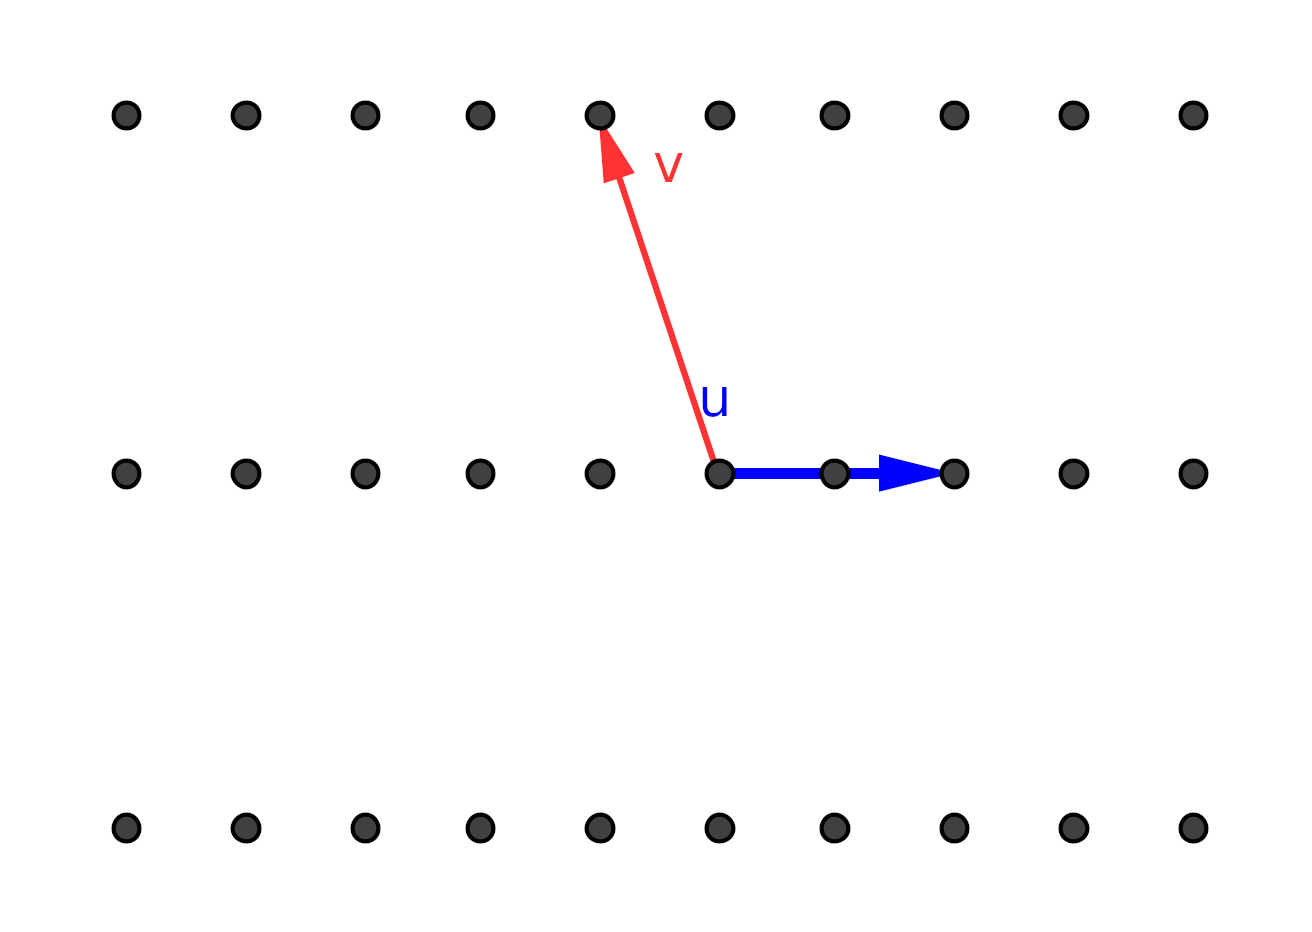
\includegraphics[]{img/lattice1}
\end{figure}

En la búsqueda de soluciones criptográficas resistentes a la computación cuántica se han encontrado útiles los siguientes problemas\cite{wickr_what_2018} de retículos:

\begin{itemize}
  \item Short Vector Problem (SVP)
  \item Short Basis Problem (SBP)
  \item Closest Vector Problem (CVP)
\end{itemize}

Llamaremos Lattice-based encryption (para ajustarnos a la bibliografía, que está en su práctica totalidad escrita en inglés) a la aplicación de este conjunto de problemas a la criptografía.

En cuanto a nuestro caso, el problema del Aprendizaje con Errores (Learn With Errors en adelante) aplicado a retículos será el núcleo de la criptografía homomórfica.

\subsection{Learn With Errors}

https://semidoc.github.io/zijlstra-lwe

\section{Generaciones}

\subsection{Pre}



\subsection{Primera generación}



\subsection{Segunda generación}

- BGV

https://eprint.iacr.org/2011/277

- BFV

https://eprint.iacr.org/2012/144

\if false
The BFV scheme cannot perform arbitrary computations on encrypted data.
    Instead, each ciphertext has a specific quantity called the `invariant noise
    budget' -- or `noise budget' for short -- measured in bits. The noise budget
    in a freshly encrypted ciphertext (initial noise budget) is determined by
    the encryption parameters. Homomorphic operations consume the noise budget
    at a rate also determined by the encryption parameters. In BFV the two basic
    operations allowed on encrypted data are additions and multiplications, of
    which additions can generally be thought of as being nearly free in terms of
    noise budget consumption compared to multiplications.
\fi

% A paper by Costache and Smart [CS16]gives some initial comparisons between BGV, BFV

- CKKS

No está descrito en el estándar, pero sí se implementa en SEAL.

https://link.springer.com/chapter/10.1007%2F978-3-319-70694-8_15

- TéCnIcA BoOtsTrApPiNg

% https://link.springer.com/chapter/10.1007/978-3-642-30057-8_1

\subsection{Tercera generación}

- GSW



- TFHE



\section{Aplicaciones}
